\documentclass{beamer}
\usecolortheme{dove}
\setbeamertemplate{navigation symbols}{}
\usepackage{amsmath,amssymb,amsfonts,amsthm, multicol, subfigure, color}
\usepackage{bm}
\usepackage{graphicx}
\usepackage{tabularx}
\usepackage{booktabs}
\usepackage{hyperref}
\usepackage{pdfpages}
\usepackage{xcolor}
\definecolor{seagreen}{RGB}{46, 139, 87}
\def\independenT#1#2{\mathrel{\rlap{$#1#2$}\mkern2mu{#1#2}}}
\newcommand\indep{\protect\mathpalette{\protect\independenT}{\perp}}
\def\log{\text{log}}
\newcommand\logit{\text{logit}}
\newcommand\iid{\stackrel{\text{iid}}{\sim}}
\newcommand\E{\text{E}}
\newcommand\V{\text{V}}
\renewcommand\P{\text{P}}
\newcommand{\Cov}{\text{Cov}}
\newcommand{\Cor}{\text{Cor}}
\newcommand\doop{\text{do}}


\usepackage{stackrel}
\usepackage{tikz}
\usetikzlibrary{arrows,shapes.arrows,positioning,shapes,patterns,calc}
\newcommand\slideref[1]{\vskip .1cm \tiny \textcolor{gray}{{#1}}}
\newcommand\red[1]{\color{red}#1}
\newcommand\blue[1]{\color{blue}#1}
\newcommand\gray[1]{\color{gray}#1}
\newcommand\seagreen[1]{\color{seagreen}#1}
\newcommand\purple[1]{\color{purple}#1}
\newcommand\orange[1]{\color{orange}#1}
\newcommand\black[1]{\color{black}#1}
\newcommand\white[1]{\color{white}#1}
\newcommand\teal[1]{\color{teal}#1}
\newcommand\magenta[1]{\color{magenta}#1}
\newcommand\Fuchsia[1]{\color{Fuchsia}#1}
\newcommand\BlueGreen[1]{\color{BlueGreen}#1}
\newcommand\bblue[1]{\textcolor{blue}{\textbf{#1}}}
\newcommand\bred[1]{\textcolor{red}{\textbf{#1}}}
\newcommand\bgray[1]{\textcolor{gray}{\textbf{#1}}}
\newcommand\bgreen[1]{\textcolor{seagreen}{\textbf{#1}}}
\newcommand\bref[2]{\href{#1}{\color{blue}{#2}}}
\colorlet{lightgray}{gray!40}
\pgfdeclarelayer{bg}    % declare background layer for tikz
\pgfsetlayers{bg,main} % order layers for tikz
\newcommand\mycite[1]{\begin{scriptsize}\textcolor{darkgray}{(#1)}\end{scriptsize}}
\newcommand{\tcframe}{\frame{
%\small{
\only<1|handout:0>{\tableofcontents}
\only<2|handout:1>{\tableofcontents[currentsection]}}
%}
}

\setbeamertemplate{footline}[frame number]

\setbeamertemplate{navigation symbols}{}

\addtobeamertemplate{footline}{
	\leavevmode%
	\hbox{%
		\begin{beamercolorbox}[wd=\paperwidth,ht=2.75ex,dp=.5ex,right,rightskip=1em]{mycolor}%
			\usebeamercolor[fg]{navigation symbols}\insertslidenavigationsymbol%
		\end{beamercolorbox}%
	}%
	\vskip0.5pt%
}{}





\usepackage[round]{natbib}
\bibliographystyle{humannat-mod}
\setbeamertemplate{enumerate items}[default]
\usepackage{mathtools}

\newcommand{\goalsframe}{\begin{frame}{Learning goals for today}
At the end of class, you will be able to:
\begin{enumerate}
\item Identify a sufficient adjustment set using the backdoor criterion
\item Assess whether selection bias may hold in a gathered sample
\end{enumerate} \vskip .2in
\end{frame}}

\title{Sufficient adjustment sets in DAGs}
\author{INFO/STSCI/ILRST 3900: Causal Inference}
\date{19 Sep 2023}

\begin{document}

\begin{frame}[noframenumbering,plain]
  \titlepage
\end{frame}



\goalsframe


\begin{frame}{Logistics}
\begin{itemize}
\item Ch 7.1 - 7.4 in Hernan and Robins 
\item Homework posted today, due Sep 28
\end{itemize}
\end{frame}


\begin{frame}
\frametitle{Open or blocked?}

How to check if a path is open or blocked:
\begin{enumerate}
    \item Traverse the path node by node 
    \item If any node is blocked, the entire path is blocked
    \item If all nodes are open, then entire path is open
\end{enumerate}

\pause 
\vspace{2em}

How to check if a node is open or blocked:
\begin{itemize}
    \item If non-collider:
    \begin{itemize}
        \item Open if it is not in the conditioning set
        \item Blocked if it is in the conditioning set
    \end{itemize} \pause
    \item If collider:
    \begin{itemize}
        \item Open if it or any of its descendants are in the conditioning set
        \item Otherwise it is blocked
    \end{itemize} \pause
\end{itemize}

\end{frame}


\begin{frame}
\frametitle{Exchangeability and DAGs}
\begin{itemize}
    \item In a \textbf{causal path}, all edges point from the treatment and toward the outcome \pause
    \item Conditional Exchangeability holds if \textbf{all} unblocked paths (given $L$) from $A$ to $Y$ are causal paths \pause
    \item The only association we observe between $A$ and $Y$ is due to causation 
\end{itemize}

\end{frame}


\begin{frame}
\frametitle{Big picture}

\begin{itemize}
     \item Find a set of variables $L$ that blocks all non-causal paths from $A$ and $Y$
     \item $L$ is called \textbf{sufficient adjustment set} \pause 
     \item \textbf{If} the DAG is true, this means $Y^{a} \indep A \mid L$ \pause
    \item Use standardization (Lecture 2-3) or inverse probability weighting (Lecture 2-4) to estimate average causal effect
\end{itemize}

\end{frame}



\begin{frame}
\frametitle{Big picture}

\begin{itemize}
     \item Find a set of variables $L$ that blocks all non-causal paths from $A$ and $Y$
     \item $L$ is called \textbf{sufficient adjustment set} \pause 
     \item \textbf{If} the DAG is true, this means $Y^{a} \indep A \mid L$ \pause
    \item Use standardization (Lecture 2-3) or inverse probability weighting (Lecture 2-4) to estimate average causal effect
\end{itemize}

\end{frame}


\begin{frame}
\frametitle{Backdoor criterion}

\begin{figure}
\begin{tikzpicture}[x = \textwidth, y = .8\textheight]
\node (a) at (.5, .45) {$A$};
\node (l) at (.3, .45) {$L$};
\node (y) at (.7, .45) {$Y$};
\draw[->, thick] (l) to[out = 45, in = 135] (y);
\draw[->, thick] (l) -- (a);
\draw[->, thick] (a) -- (y);
\only<2->{
\draw[->, thick, red] (l) to[out = 45, in = 135] (y);
\draw[->, thick, red] (l) -- (a);}
\end{tikzpicture}
\end{figure}
\only<2->{
{\color{red} Backdoor path} starts with an edge pointing in to $A$ and ends at $Y$
}

\vspace{1em}
\only<3->{
A set of variables satisfies the backdoor criterion if\pause 
\begin{enumerate}
     \item Blocks all backdoor paths \pause
     \item Does not contain any descendant of $A$
\end{enumerate}
}

\vspace{1em}
\only<4->{
Sets that satisfy the backdoor criterion are sufficient adjustment sets! 
}
\end{frame}


\begin{frame}
\frametitle{Exercise}
Researchers may be interested in the effect of fluoroquinolones, a class of antibiotics, on epilepsy\footnote{Example from ``Using Causal Diagrams to Improve the Design and Interpretation of Medical Research'' (Etminan et. al. 2020, Chest) }

\begin{figure}[t]
	\centering
	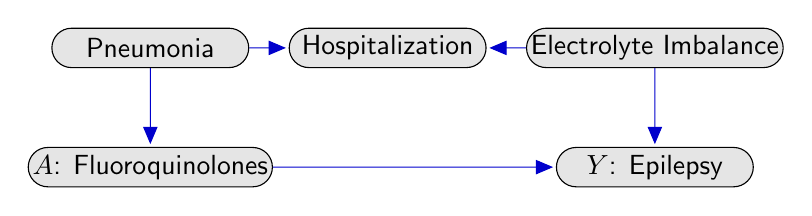
\begin{tikzpicture}[->,>=triangle 45,shorten >=1pt,
	auto, main node/.style={rounded rectangle,inner sep=0pt,fill=gray!20,draw,font=\sffamily,
		minimum width = 2.5cm, minimum height = .5cm}]

    \node[main node] (X) {$A$: Fluoroquinolones};
    \node[main node] (U1) [above = 1cm of X] {Pneumonia};
\node[main node] (H) [right = .5cm of U1] {Hospitalization};
    \node[main node] (U2) [right = .5cm of H] {Electrolyte Imbalance};
    \node[main node] (Y) [below = 1cm of U2] {$Y$: Epilepsy};

    \path[color=black!20!blue,style={->}]
	(X) edge node {} (Y)
	(U1) edge node {} (X)
	(U1) edge node {} (H)
	(U2) edge node {} (H)
	(U2) edge node {} (Y)
	;
	

	\end{tikzpicture}
		
\end{figure}

\vspace{1em}
\begin{itemize}
    \item Does a sufficient adjustment set exist? If so, what is it?
\end{itemize}


\end{frame}


\begin{frame}
\frametitle{Exercise}
Researchers may be interested in the effect of fluoroquinolones, a class of antibiotics, on epilepsy\footnote{Example from ``Using Causal Diagrams to Improve the Design and Interpretation of Medical Research'' (Etminan et. al. 2020, Chest) }

\begin{figure}[t]
	\centering
	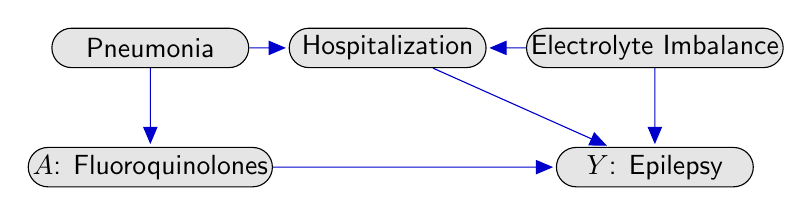
\begin{tikzpicture}[->,>=triangle 45,shorten >=1pt,
	auto, main node/.style={rounded rectangle,inner sep=0pt,fill=gray!20,draw,font=\sffamily,
		minimum width = 2.5cm, minimum height = .5cm}]

    \node[main node] (X) {$A$: Fluoroquinolones};
    \node[main node] (U1) [above = 1cm of X] {Pneumonia};
\node[main node] (H) [right = .5cm of U1] {Hospitalization};
    \node[main node] (U2) [right = .5cm of H] {Electrolyte Imbalance};
    \node[main node] (Y) [below = 1cm of U2] {$Y$: Epilepsy};

    \path[color=black!20!blue,style={->}]
	(X) edge node {} (Y)
	(U1) edge node {} (X)
	(U1) edge node {} (H)
	(U2) edge node {} (H)
	(U2) edge node {} (Y)
        (H) edge node {} (Y)
	;
	

	\end{tikzpicture}
		
\end{figure}

\vspace{1em}
\begin{itemize}
    \item Does a sufficient adjustment set exist? If so, what is it?
\end{itemize}


\end{frame}

\begin{frame}
\frametitle{Exercise}

Researchers may be interested in the effect of diabetes on cardiac Ischemia\footnote{Example from ``Using Causal Diagrams for Biomedical Research'' (Kyriacou et. al. 2023, Annals of Emergency Medicine
) }

\begin{figure}
\begin{tikzpicture}[x = \textwidth, y = .8\textheight]
\node (a) at (.3, .45) {Diabetes};
\node (y) at (.7, .45) {Cardiac ischemia};
\node (age) at (.45, .6) {Age};
\node (obs) at (.4, .75) {Obesity};
\node (hyp) at (.65, .75) {Hypertension};

\draw[->, thick] (a) -- (y);
\draw[->, thick] (age) -- (a);
\draw[->, thick] (age) -- (y);
\draw[->, thick] (obs) -- (a);
\draw[->, thick] (obs) -- (y);
\draw[->, thick] (obs) -- (hyp);
\draw[->, thick] (hyp) -- (y);

\end{tikzpicture}
\end{figure}

\vspace{1em}
\begin{itemize}
    \item Does a sufficient adjustment set exist? If so, what is it?
\end{itemize}

\end{frame}



\begin{frame}
\frametitle{Selection Bias}

\begin{itemize}
    \item Sufficient adjustment set to close backdoor paths \pause
    \item Does not always mean conditioning on more things

\begin{figure}
\begin{tikzpicture}[x = \textwidth, y = .8\textheight]
\node (a) at (.3, .45) {$A$};
\node (z1) at (.3, .6) {$Z_1$};
\node (z2) at (.5, .525) {$Z_2$};
\node (z3) at (.7, .6) {$Z_3$};
\node (y) at (.7, .45) {$Y$};
\draw[->, thick] (z3) -- (y);
\draw[->, thick] (z1) -- (a);
\draw[->, thick] (z1) -- (z2);
\draw[->, thick] (z3) -- (z2);
\draw[->, thick] (a) -- (y);
\end{tikzpicture}
\end{figure}
        
\end{itemize}


\end{frame}

\begin{frame}
\frametitle{Selection Bias}
In some settings, certain variables may already be ``conditioned on''  \pause

\vspace{1em}
Researchers may be interested in the effect of fluoroquinolones, a class of antibiotics, on epilepsy\footnote{Example from ``Using Causal Diagrams to Improve the Design and Interpretation of Medical Research'' (Etminan et. al. 2020, Chest) }

\begin{figure}[t]
	\centering
	\begin{tikzpicture}[->,>=triangle 45,shorten >=1pt,
	auto, main node/.style={rounded rectangle,inner sep=0pt,fill=gray!20,draw,font=\sffamily,
		minimum width = 2.5cm, minimum height = .5cm}]

    \node[main node] (X) {$A$: Fluoroquinolones};
    \node[main node] (U1) [above = 1cm of X] {Pneumonia};
    \only<2>{\node[main node] (H) [right = .5cm of U1] {Hospitalization};}
    \only<3>{\node[main node, rectangle, fill = white] (H) [right = .5cm of U1] {Hospitalization};}
    \node[main node] (U2) [right = .5cm of H] {Electrolyte Imbalance};
    \node[main node] (Y) [below = 1cm of U2] {$Y$: Epilepsy};

    \path[color=black!20!blue,style={->}]
	(X) edge node {} (Y)
	(U1) edge node {} (X)
	(U1) edge node {} (H)
	(U2) edge node {} (H)
	(U2) edge node {} (Y)
	;
	

	\end{tikzpicture}
		
\end{figure}


\end{frame}

\begin{frame}
\frametitle{Selection Bias}


\begin{figure}[t]
	\centering
	\begin{tikzpicture}[->,>=triangle 45,shorten >=1pt,
	auto, main node/.style={rounded rectangle,inner sep=0pt,fill=gray!20,draw,font=\sffamily,
		minimum width = 2.5cm, minimum height = .5cm}]

    \node[main node] (X) {$A$: Play sport};
    \node[main node] (Y) [right = 2.5cm of X] {$Y$: Good Grades};
   \only<3-4>{ \node[main node] (Z) [below right= 1cm of X] {College}; }
    \only<5-6>{ \node[main node, rectangle, fill = white] (Z) [below right= 1cm of X] {College}; }

    \path[color=black!20!blue,style={->}]
	(X) edge node {} (Y)
	;
 \only<3->{\path[color=black!20!blue,style={->}]
	(X) edge node {} (Z)
 	(Y) edge node {} (Z)
	;}
	

	\end{tikzpicture}
		
\end{figure}
\vspace{2em}
\only<4>{
\[A \indep Y^{a} \]
}
\only<6>{
\[A \indep Y^{a} \mid \text{College}\]
}




\end{frame}

\begin{frame}
\frametitle{Selection Bias}

\begin{itemize}
    \item Gathered data is typically restricted to some group \pause
    \item This may implicitly condition on a variable \pause
    \item May open non-causal paths
\end{itemize}

\end{frame}



\begin{frame}
\frametitle{Takeaways}
\begin{itemize}
    \item Drawing the DAG makes your causal assumptions clear to yourself and others \pause
    \item Clear rules for what to adjust for \textbf{if the DAG is true}
    \begin{itemize}
        \item \textbf{Sufficient adjustment set} blocks all non-causal paths
        \item If it exists, use standardization or IPW to estimate causal effect
        \item If it does not exist, consider gathering more variables
    \end{itemize}
    \item Carefully consider the data gathering process \pause 
    \item Causal claims come from assumptions + data  
\end{itemize}


\end{frame}


\goalsframe


\end{document}

